\documentclass[a4paper,english]{G2-105}
\usepackage[T1]{fontenc}
\usepackage{multirow}
\usepackage{graphicx}

\begin{document}
\abstract{Аннотация}
\par Документ представляет собой техническое задание к выпускной работе бакалавра на тему «Портирование сверточной нейросети на ARM архитектуру с ограниченными вычислительными ресурсами и ресурсами памяти», выполненную студентом группы ИВТ-461, Мельниковым Тимофеем Алексеевичем.
\par Составлено и оформлено согласно ГОСТ 19.201-78.
\par Объём технического задания составил \totalpages~страниц и включает \totalfigures~рисунка и \totaltables~таблицы. 
\VSTUInitializeTZ
\tableofcontents
\newpage

\chaptertz{Введение}

\section{Наименование программы}
\par Разработке подлежит программный продукт, представляющий собой клиент-серверное приложение для детектирования объектов на изображении, используя сверточную нейронную сеть, на устройствах с ARM-архитектурой.
Полное наименование приложения --- "Приложение для прямного прохода сверточной нейронной сети на ARM-устройстве". Краткое наименование --- "C.H.I.P. Vision". Далее используется краткое название --- Приложение.

\section{Область применения}
\par Приложение предназначено для использования компьютерного зрения, основанного на машинном обучении, в встаиваемых системах с архитектурой ARM.

\chaptertz{Основание для разработки}
\ttl
\section{Документ, на основании которых ведется проектирование}
\par Разработка ведется на основании задания на выполнение выпускной квалификационной работы бакалавра по направлению «Информатика и вычислительная техника».

\section{Организация, утвердившая этот документ, и дата его утверждения}
Задание на выполнение выпускной квалификационной работы бакалавра выдано к.т.н., доцентом кафедры «Системы автоматизированного проектирования и поискового конструирования» Катаевым А. В.
\par Задание выдано «\_\_» \_\_\_\_\_\_\_\_2016 г.
\par Срок окончания работ «\_\_» \_\_\_\_\_\_\_\_2017 г.


\section{Наименование и условное обозначение темы разработки}
\par Наименование темы разработки --- Приложение осуществляющее прямой проход сверточной нейронной сети на устройстве с ARM-архитектурой.

\chaptertz{Назначение разработки}
\par Приложение предназначено для исследования вычислений сверточных нейроных сетей на ARM-архитектуре, выполняющих детектирование объектов на изображнии, и визуализации выполненых вычислений на клиентском компьютере.

\chaptertz{Требование к программе}
\section{Требования к функциональным характеристикам}
\par Приложение разделено на клиентскую и серверную части. Серверная часть запускается на ARM-устройстве и выполняет детектирование объектов на изображении, используя сверточные нейронные сети, и функции для работы с клиентом. Клиетская часть запускается на персональном компьютере пользователя и предоставляет возможность подключаться к серверной программе, выбирать изображение для детектирования на нем объектов и просматривать результаты работы детектирования объектов. 
\subsection{Требования к составу выполняемых функций}
\par Серверная программа должна выполнять следующие группы функций:
\begin{itemize}
\item Функции работы с клиентом;
\item Функции парсинга и сериализации конфигураций нейронной сети;
\item Функции детектирования объектов на изображении.
\end{itemize}
~\ 
\par Для работы с клиентом должны быть реализованы следующие функции:
\begin{itemize}
\item Создание сокета для входных подключений;
\item Связка сокета с сетевым оборудованием;
\item Создание клиентского сокета, после подключения клиента;
\item Ожидание и выполнение команд клиента.
\end{itemize}
~\ 
\par Для реализации парсинга и сериализации данных должны быть реализованы следующие функции:
\begin{itemize}
\item Парсинг и сериализация меток детектируемых объектов. Формат файла меток представлен в приложении 1, рисунок ~\ref{network_cfg};
\item Парсинг и сериализация файла конфигурации сверточной нейронной сети YOLO. Файл конфигурации представлен в приложении 1, рисунок ~\ref{network_cfg};
\item Парсинг и сериализация весов сверточной нейронной сети Tiny YOLO. Веса хранятся последовательно в двоичном формате.
\end{itemize}
~\ 
\par Для детектирования объектов на изображении необходимо реализовать следущие функции:
\begin{itemize}
\item Сериализация изображения для детектирования объектов на нем;
\item Прямой проход следующих слоев:
\begin{enumerate}
\item Сверточный слой;
\item Слой объединения;
\item Слой контуров.
\end{enumerate}
\item Активация следующих нелинейных функций:
\begin{enumerate}
\item Жеская пороговая функция;
\item Линейная функция;
\item Leaky функция.
\end{enumerate}
\item Локализация найденных объектов;
\item Отрисовка меток и границ объектов.
\end{itemize}
~\ 
\par Клиентская программа должна выполнять следующие группы функций:
\begin{itemize}
\item Функции работы с сервером;
\item Функции взаимодействия с пользователем.
\end{itemize}
~\ 
\par Для работы с сервером необходимо реализовать следущие функции:
\begin{itemize}
\item Получение хоста сервера;
\item Соединение с сервером.
\end{itemize}
~\ 
\par Для взаимодействием с пользователем необходимо реализовать следущие функции:
\begin{itemize}
\item Соединение с сервером;
\item Выбор изображения для детектирования объектов на нем;
\item Отображение процесса работы прямого прохода Tiny YOLO;
\item Отображение результатов прямого прохода Tiny YOLO. А именно изображение с метками и отрисованными границами объектов.
\end{itemize}
~\ 
\par Для осуществления передачи данных между клиентом и сервером необходимо реализовать интерфес работы с сокетами. Данный модуль является общим для клиента и сервера и должен выполнять следующие функции:
\begin{itemize}
\item Отправка сообщения;
\item Получение сообщения;
\item Отправка изображения;
\item Получение изображения.
\end{itemize} 

\section{Организация входных и выходных данных}
\subsection{Входные данные}
\par Входными данными для клиентской части приложения является изображение в формате png или jpg. Любой файл иного формата, но с расширением png или jpg, открываться не должен. В процессе вычислений серверная программа должна отправлять клиенту информацию о пройденных этапах вычислений. В приложении 2 описан процесс обмена данными между клиентской и серверной частями.
\par Входными данными для серверной части приложения является сообщение от клиента. В таблице ~\ref{input} приведены входные данные запрашиваемые сервером в зависимости от полученного сообщения.
\begin{longtable}{|c|c|}
    \caption{Входные данные серверной части приложения} \label{input} \\ \hline
    Сообщение        & Входные данные            \\ \hline \endhead
    "yolo"           & изображение в формате png \\ 
                     & или jpeg в байтовом       \\
                     & представлении             \\ \hline
    "exit"           & ---                       \\ \hline
    другое сообщение & сообщение с корректной    \\  
    	                 & командой ("yolo" или "exit") \\
\end{longtable}

\subsection{Выходные данные}
\par Выходными даными приложения является изображение с метками найденных объектов. Каждый найденный объект должен быть замкнут прямоугольник. Подробная информация об визуализации выходного изображения представлена в приложении 3.
\par Клиентская часть программы должна иметь текстовый браузер для вывода информации о основных этапах работы серверной части приложения. В приложении 2 на диаграмме последовательности показано, какая информация о этапах серверной части должна быть выведена.
\par В таблице ~\ref{output} приведены выходные данные серверной части, в зависимости от сообщения.
\par Серверная часть приложения должна выводить в стандарстный поток ввода/вывода основную информацию о этапах работы. В приложении 2 на диаграмме последовательности показаны информационные блоки, которые должны выводится в страндартый поток ввода/вывода.
\begin{longtable}{|c|c|}
    \caption{Выходные данные серверной части приложения} \label{output} \\ \hline
    Сообщение        & Входные данные            \\ \hline \endhead
    "yolo"           & изображение в формате png \\ 
                     & с отрисованными метками и \\
                     & границами объектов в      \\
                     & байтовом представлении    \\ \hline
    "exit"           & ---                       \\ \hline
    другое сообщение & ---                       \\  
    	                 & ---                       \\
\end{longtable}

\section{Требования к надежности}
\subsection{Требования к надежному функционированию}
Надежное функционирование приложения должно быть обеспечено выполнением Заказчиком совокупности организационно-технических мероприятий, перечень которых приведен ниже:
\begin{itemize}
\item организацией бесперебойного питания технических средств
\item использованием лицензионного программного обеспечения
\end{itemize}
\subsection{Время восстановления после отказа}
\par Время восстановления после отказа, вызванного неисправностью технических средств, фатальным сбоем (крахом) операционной системы, не должно превышать времени, требуемого на устранение неисправностей технических средств и переустановки программных средств.

\subsection{Требования к составу и параметрам технических средств}
Эксплуатация клиентской части приложение конечным пользователем подразумевает у него наличие Linux-подобной операционной системы с подключением к интернету. В операционной системе должна быть предустановленна библиотека Qt 5.8.0.
\par Ниже приведены требования к техническим средствам компьютера:
\begin{itemize}
\item процессор мощностью не менее 1 ГГц;
\item оперативная память не менее 512 Мб;
\item свободное место не менее 100 Мб;
\item устройства взаимодействия с пользователем — клавиатура, мышь и
монитор.
\end{itemize}
~\ 
\par Запуск серверной части приложения должен осущетвлятся на встраиваемом решении с процессором ARM. Должны поддрерживаться следущие семейства процессоров:
\begin{itemize}
\item ARM7
\item ARM9
\item Cortex A
\end{itemize}
~\ 
\par Устройство должно обладать Linux-подобной операционной системой с подключением к интернету.
\par Ниже приведены требования к техническим средствам компьютера:
\begin{itemize}
\item процессор мощностью не менее 60 МГц;
\item оперативная память не менее 512 Мб;
\item свободное место не менее 500 Мб;
\item устройства взаимодействия с пользователем — клавиатура и монитор.
\end{itemize}

\section{Требования к информационной и программной совместимости}
\subsection{Требования к методам решения}
\par Методы решения должны обеспечивать выполнение всех этапов проектирования приложения в соответствии с их порядком и сроками выполнения, указанными в разделе 7 данного документа.
\subsection{Требования к языкам программирования}
\par Клиентская часть должна быть написана на языке C/C+.
\par Серверная часть должна быть написана на языке C. Серверная часть не должна содержать внешних зависимостей. Разрешается использовать только системные библиотеки.

\chaptertz{Требования к программной документации}
\par К приложению прилагается следующая документация:
\begin{itemize}
\item Техническое задание согласно ГОСТ 19.201-78;
\item Пояснительная записка.
\end{itemize}

\chaptertz{Стадии и этапы разработки}
\section{Стадии разработки}
\par Разработка должна включать следующие стадии:
\begin{itemize}
\item Изучение используемого фреймворка нейронных сетей
«darknet» (ноябрь-декабрь);
\item Изучение архитектур сверточных нейронных сетей: «YOLO»,
Tiny YOLO»;
\item Разработка технического задания (февраль);
\item Рабочее проектирование (февраль-март);
\item Реализация и тестирование программы (апрель-май)
\end{itemize}

\section{Этапы разработки}
\par На стадии изучения фреймворка «darknet» должны быть
выполнены следующие этапы:
\begin{itemize}
\item Изучить функции работы с изображениеми и способ
представления изображения;
\item Изучить функции чтения конфигурации нейронной сети,
весовых коэффициентов;
\item Изучить построение архитектуры работы слоев и связи между
ними.
\end{itemize}
~\                    
\par На стадии разработки технического задания должны быть
выполнены следующие этапы:
\begin{itemize}
\item Разработка технического задания;
\item Согласование и утверждение технического создания.
\end{itemize}
~\ 
\par На стадии рабочего проектирования должны быть выполнены
перечисленные ниже этапы:
\begin{itemize}
\item Разработка клиентской части приложения;
\item Разработка серверной части приложения;
\item Реализация интерфейса взаимодействия клиентской и серверной части.
\end{itemize}
~\ 
\par На стадии реализации программы должны быть выполнены
перечисленные ниже этапы:
\begin{itemize}
\item Реализация вертикального прототипа;
\item Доработка прототипа до конечного продукта.
\end{itemize}
~\ 
\par На стадии тестирования программы должны быть выполнены
перечисленные ниже этапы:
\begin{itemize}
\item Анализ корректности вычислений при прямом проходе сверточной нейронной сети Tiny YOLO;
\item Анализ быстродействия программы вычислений на ARM-устройстве.
\end{itemize}

\chaptertz{Порядок контроля и приемки}
\section{Виды испытаний}
\par Испытания программы и верификация документации должны проводиться в организации заказчика.
\par Приемо-сдаточные испытания приложения должны производиться доцентом кафедры САПРиПК Катаевым А. В. 
\par Программа должна соответствовать всем требованиям, изложенным в Техническом задании.
\section{Общие требования к приемке}
\par Приемка программы должна производиться доцентом кафедры
САПРиПК Катаевым А. В.
\par Программа должна считаться годной для приемки, если в процессе
тестирования заказчиком она удовлетворяет всем пунктам данного
технического задания.

\appendixtz{Формат конфигруационных файлов нейронной сети}
\begin{figure} 
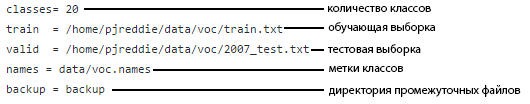
\includegraphics[width = \linewidth]{metki.png}
\caption{Данные о выборке и метках объектов}\label{met}
\end{figure}
\begin{figure} 
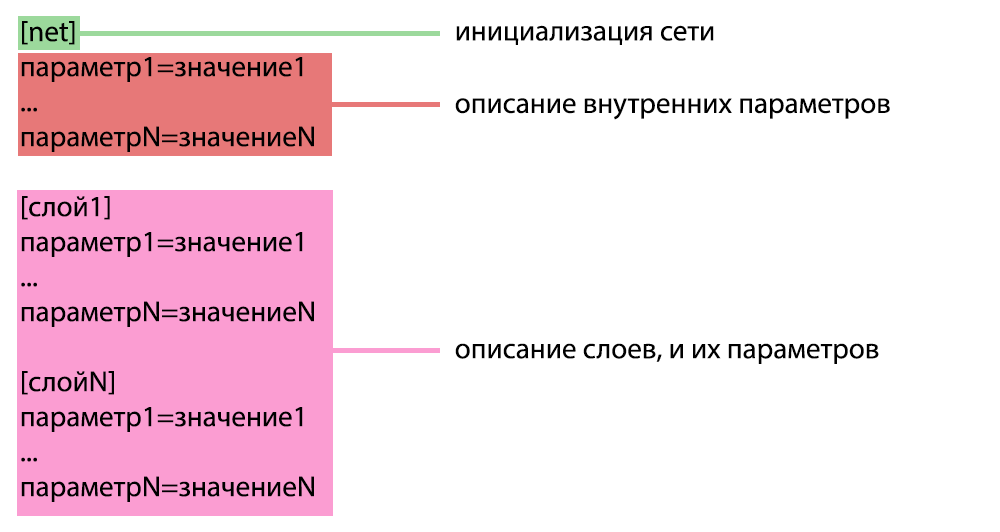
\includegraphics[width = \linewidth]{network_cfg.png}
\caption{Конфигурационный файл нейронной сети}\label{network_cfg}
\end{figure}

\appendixtz{Диаграмма последовательности}
\begin{figure} 
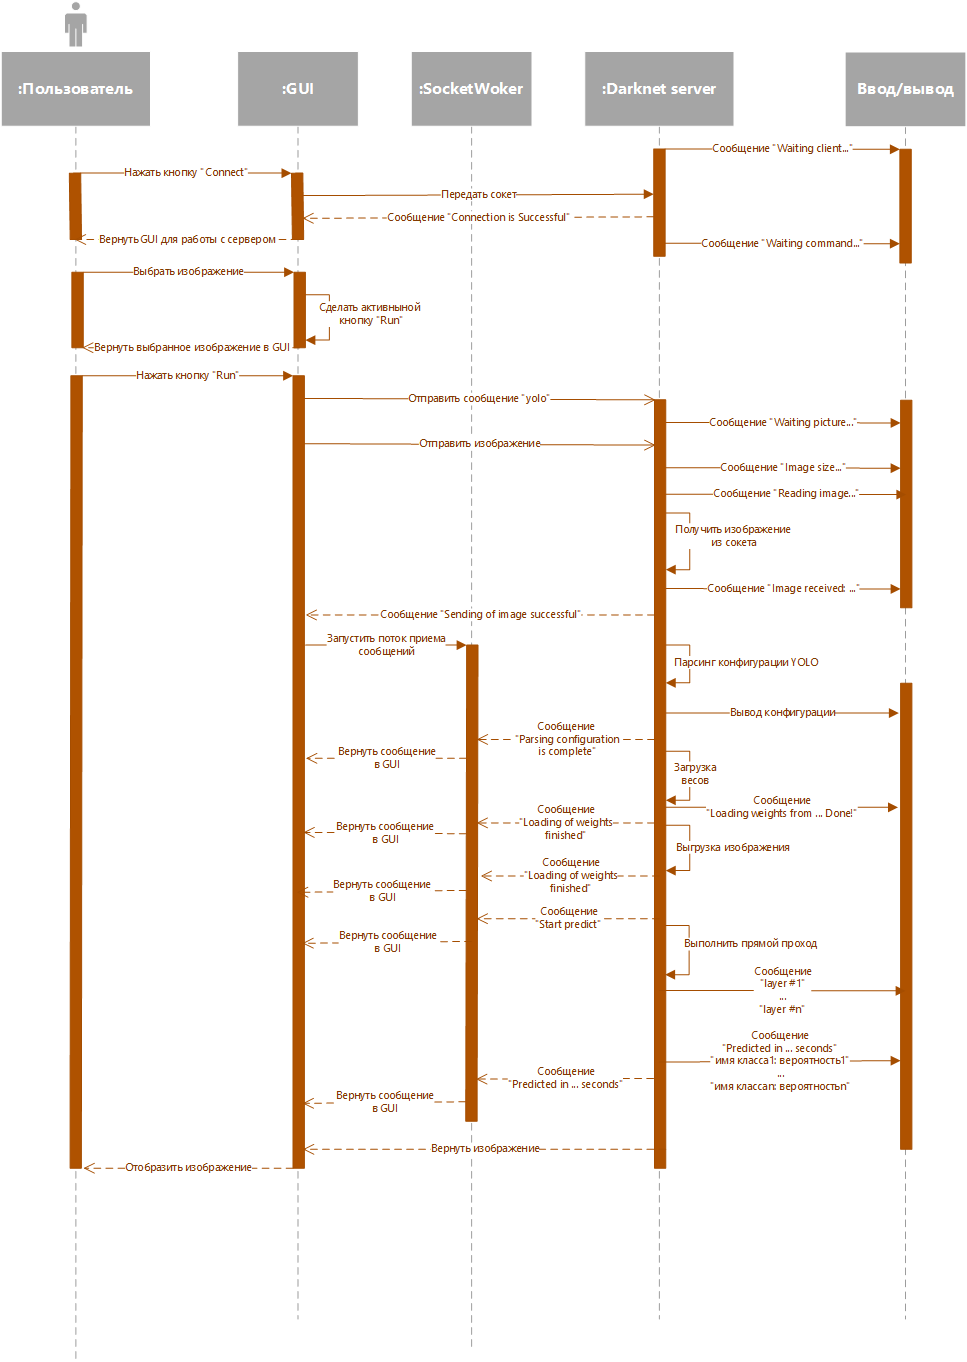
\includegraphics[width = 0.8 \linewidth]{sequence.png}
\caption{Диаграмма последовательности}\label{seq}
\end{figure}

\appendixtz{Визуализация локализации объектов}
\begin{figure} 
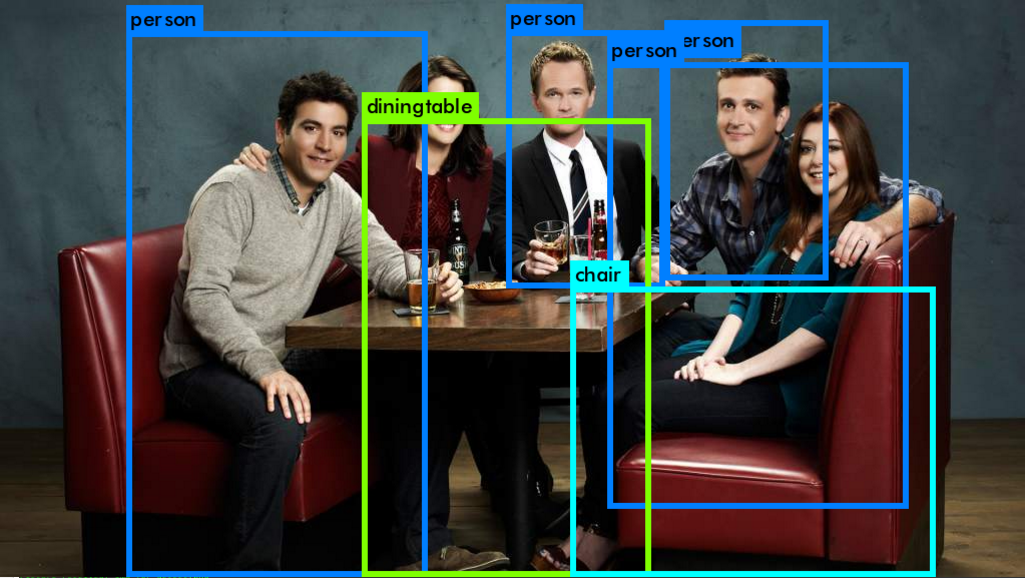
\includegraphics[width = \linewidth]{photo.png}
\caption{Метки и границы объектов}\label{photo}
\end{figure}


\appendixtz{Макеты экранных форм}
\begin{figure} 
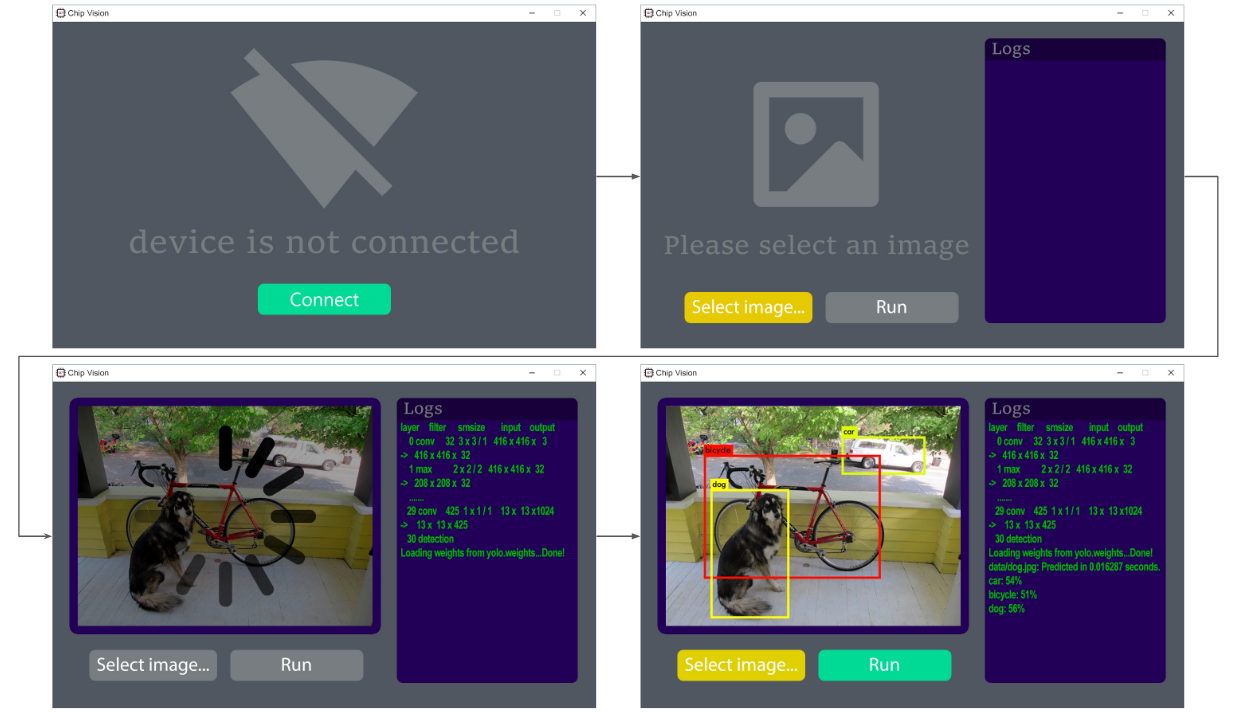
\includegraphics[width = \linewidth]{screens.png}
\caption{Макеты экранных форм}\label{photo}
\end{figure}


\end{document}
